% By J. Leon, Beerware licence is acceptable...
\documentclass[tikz,border=10pt]{standalone}
\usepackage{tikz}
\usetikzlibrary{positioning, fit, arrows.meta, shapes}

\begin{document}

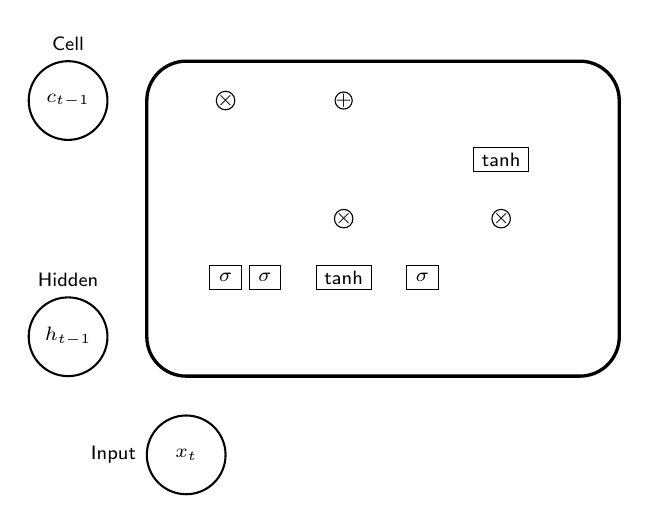
\begin{tikzpicture}[
    % GLOBAL CFG
    font=\sf \scriptsize,
    >=LaTeX,
    % Styles
    cell/.style={% For the main box
        rectangle, 
        rounded corners=5mm, 
        draw,
        very thick,
        },
    operator/.style={%For operators like +  and  x
        circle,
        draw,
        inner sep=-0.5pt,
        minimum height =.2cm,
        },
    function/.style={%For functions
        ellipse,
        draw,
        inner sep=1pt
        },
    ct/.style={% For external inputs and outputs
        circle,
        draw,
        line width = .75pt,
        minimum width=1cm,
        inner sep=1pt,
        },
    gt/.style={% For internal inputs
        rectangle,
        draw,
        minimum width=4mm,
        minimum height=3mm,
        inner sep=1pt
        },
    mylabel/.style={% something new that I have learned
        font=\scriptsize\sffamily
        },
    ArrowC1/.style={% Arrows with rounded corners
        rounded corners=.25cm,
        thick,
        },
    ArrowC2/.style={% Arrows with big rounded corners
        rounded corners=.5cm,
        thick,
        },
    ]

%Start drawing the thing...    
    % Draw the cell: 
    \node [cell, minimum height =4cm, minimum width=6cm] at (0,0){} ;



    % Draw activation functions
    \node [gt] (sigma_f) at (-2,-0.75) {$\sigma$};
    \node [gt] (sigma_i) at (-1.5,-0.75) {$\sigma$};
    \node [gt, minimum width=0.7cm] (tanh_c) at (-0.5,-0.75) {tanh};
    \node [gt] (sigma_o) at (0.5,-0.75) {$\sigma$};
    \node [gt, minimum width=0.7cm] (tanh_end) at (1.5,0.75) {tanh};

   % Draw multiplication and addition operators
    \node [operator] (mux_conveyor) at (-2,1.5) {$\times$};
    \node [operator] (add_conveyor) at (-0.5,1.5) {+};
    \node [operator] (mux_i_and_c) at (-0.5,0) {$\times$};
    \node [operator] (mux_end) at (1.5,0) {$\times$};


    % Draw External inputs? named as basis c,h,x
    \node[ct, label={[mylabel]Cell}] (c) at (-4,1.5) {$c_{t-1}$};
    \node[ct, label={[mylabel]Hidden}] (h) at (-4,-1.5) {$h_{t-1}$};
    \node[ct, label={[mylabel]left:Input}] (x) at (-2.5,-3) {$x_t$};

    % Draw External outputs? named as basis c2,h2,x2
%    \node[ct, label={[mylabel]Label1}] (c2) at (4,1.5) {$c_t$};
%    \node[ct, label={[mylabel]Label2}] (h2) at (4,-1.5) {$h_t$};
%    \node[ct, label={[mylabel]left:Label3}] (x2) at (2.5,3) {$h_t$};

% Start connecting all.
    %Intersections and displacements are used. 
    % Drawing arrows    
%    \draw [ArrowC1] (c) -- (mux_conveyor) -- (add_conveyor) -- (c2);

    % Inputs
%    \draw [ArrowC2] (h) -| (sigma_o);
%    \draw [ArrowC1] (h -| sigma_f)++(-0.5,0) -| (sigma_f); 
%    \draw [ArrowC1] (h -| sigma_i)++(-0.5,0) -| (sigma_i);
%    \draw [ArrowC1] (h -| tanh_c)++(-0.5,0) -| (tanh_c);
%    \draw [ArrowC1] (x) -- (x |- h)-| (tanh_c);

    % Internal
%    \draw [->, ArrowC2] (sigma_f) -- (mux_conveyor);
%    \draw [->, ArrowC2] (sigma_i) |- (mux_i_and_c);
%    \draw [->, ArrowC2] (tanh_c) -- (mux_i_and_c);
%    \draw [->, ArrowC2] (sigma_o) |- (mux_end);
%    \draw [->, ArrowC2] (mux_i_and_c) -- (add_conveyor);
%    \draw [->, ArrowC1] (add_conveyor -| tanh_end)++(-0.5,0) -| (tanh_end);
%    \draw [->, ArrowC2] (tanh_end) -- (mux_end);

    %Outputs
%    \draw [-, ArrowC2] (mux_end) |- (h2);
%    \draw (c2 -| x2) ++(0,-0.1) coordinate (i1);
%    \draw [-, ArrowC2] (h2 -| x2)++(-0.5,0) -| (i1);
%    \draw [-, ArrowC2] (i1)++(0,0.2) -- (x2);

\end{tikzpicture}
\end{document}